\section{Results}
Using an exposure of 34~kg of liquid xenon and 224.6~live days of data a yield of 764 events is observed  in the region of interest,
this is compatible with the expectation of $756 \, \pm \, 5^{(stat.)} \, \pm 55^{(syst.)}$ events from the background only hypothesis. 
Figure~\ref{fig:dataVSbkg} shows how these events are distributed in the region of interest, the bottom panel shows the ratio
between data and expected background, where the gray and orange shaded areas represent respectively statistical and systematic uncertainty 
on the background expectation.
%The distribution of events from data are compared to the background expectation in Figure~\ref{fig:dataVSbkg} and with the relative
%uncertainties.  

This result is interpreted via a binned profiled likelihood approach by means of the test statistic $\tilde{q}$
and its asymptotic distributions described in \cite{asympt}. 
Assuming  an isothermal WIMP halo with a local density of $\rho_{\chi} \, = \, 0.3$~$GeV/cm^3$ , a local circular velocity of $v_0 \,= \, 220$~km/s, and a galactic escape velocity of $v_{esc} \, = \, 544$ km/s, 
\textcolor{blue}{other assumptions...,} a 90\% CL$_s$~\cite{cls} confidence level limit is  
computed on the spin dependent inelastic WIMP-nucleon cross section, $\sigma_{inel}$, as a function of the WIMP mass, $m_{\chi}$, and shown in Figure~\ref{fig:limits}.
The expected median sensitivity is reported with its relative one (green area) and two (yellow area) standard deviation uncertainty.
A  limit is set on $\sigma_{inel}$ to $3.3 \times 10^{-38} ~cm^{2}$ at 90\% CL$_s$ confidence level for a WIMP of mass 100~GeV. This limit is compared with
\textcolor{blue}{decide which other experiment to plot.}

\newpage
\begin{figure}[t!]
  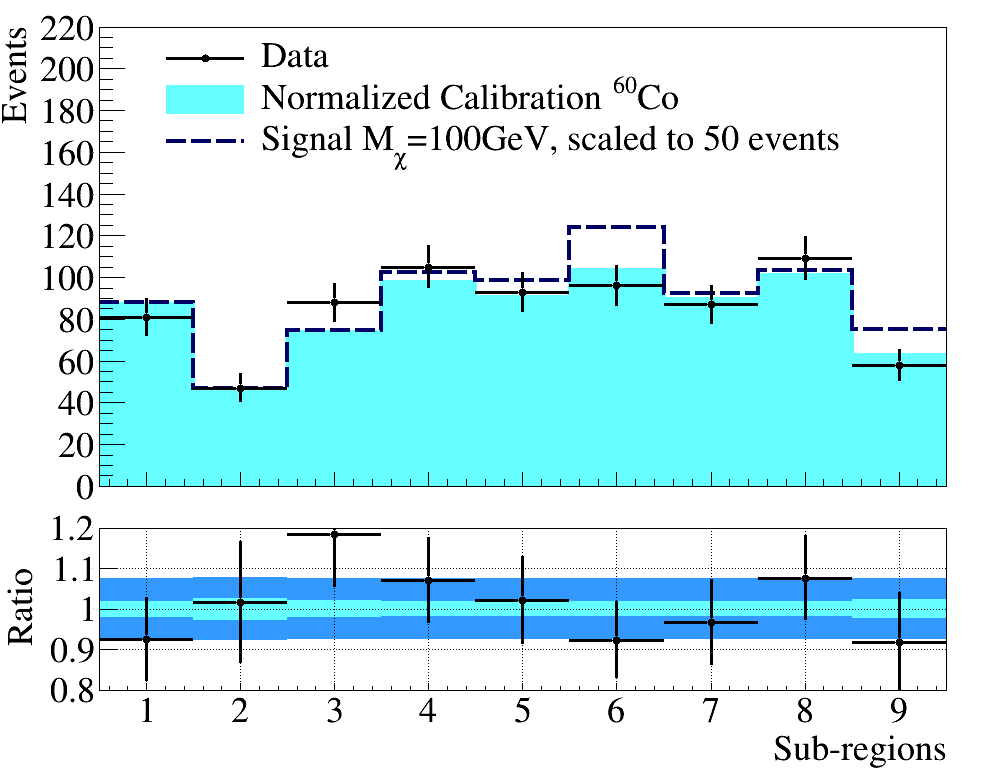
\includegraphics[width=\linewidth]{images/data_vs_bkg.png}
  \caption{Results, comparison between data and expected background.}
  \label{fig:dataVSbkg}
\end{figure}

\begin{figure}[h]
  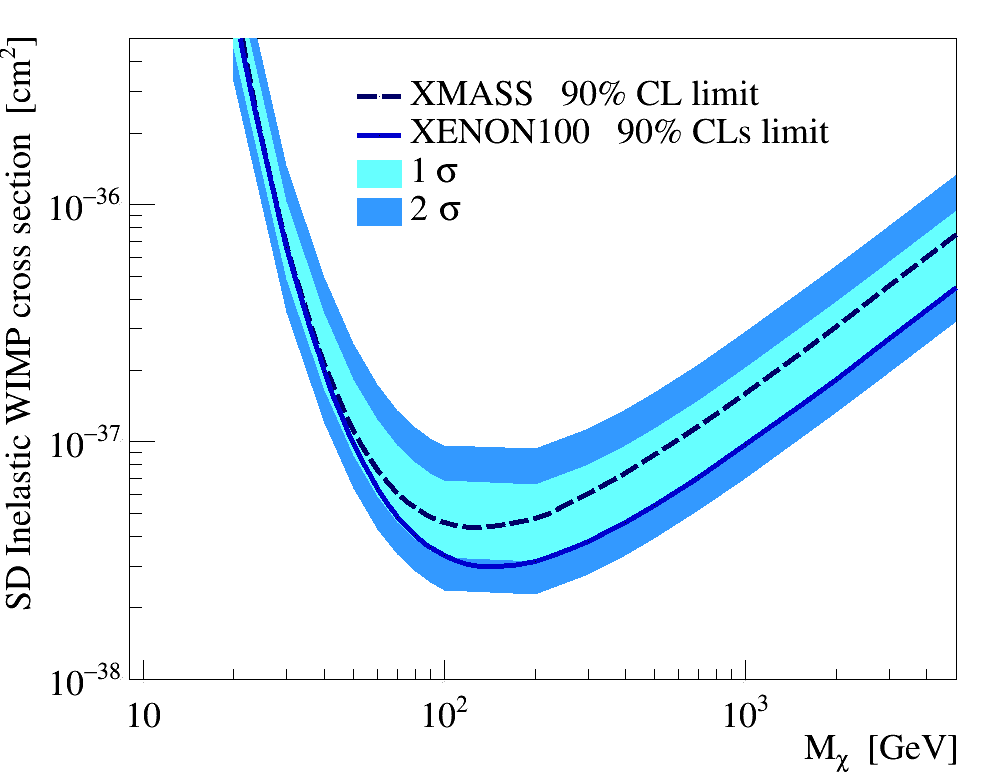
\includegraphics[width=\linewidth]{images/limit_reb.png}
  \caption{Observed and expected limits.}
  \label{fig:limits}
\end{figure}


\newpage
